%label:"fig:ExtendingByVanishingPath"
%type:"figure"
%name:"extending by vanishing path"
%caption:"A vanishing path determines a method for extending Lagrangians belonging to the Fukaya-Seidel category near a critical value to the Fukaya-Seidel category of $(Y, W)$."
%parent:"art_ComparisonToBSide"


    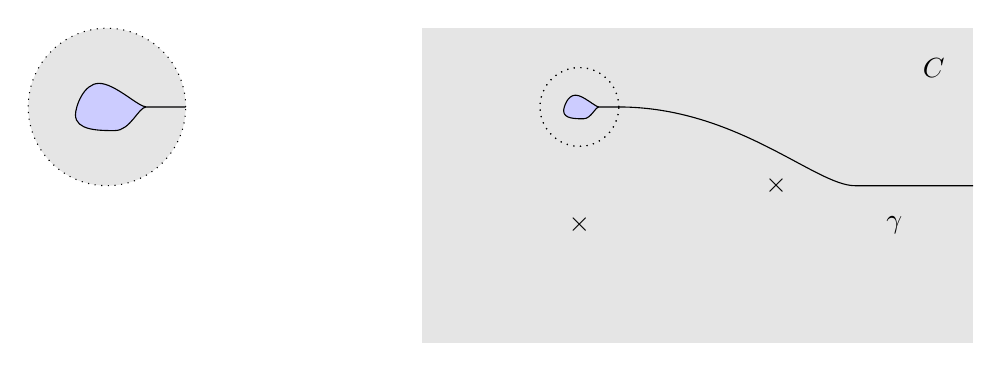
\begin{tikzpicture}

        \fill[gray!20] (-3,2.5) rectangle (4,-1.5);
        
        
        \node at (3.5,2) {$\mathbb{C}$};
        
        
        \node at (-1,0) {$\times$};
        \node at (1.5,0.5) {$\times$};
        \node at (-1,1.5) {$\times$};
        \draw[dotted]  (-1,1.5) ellipse (0.5 and 0.5);
        
        \begin{scope}[]
        \draw[dotted, fill=gray!20] (-7,1.5) ellipse (1 and 1);
        \draw[fill=blue!20] (-6,1.5) .. controls (-6.1,1.5) and (-6.4,1.5) .. (-6.5,1.5) .. controls (-6.6,1.5) and (-6.9,1.8) .. (-7.1,1.8) .. controls (-7.3,1.8) and (-7.4,1.5) .. (-7.4,1.4) .. controls (-7.4,1.2) and (-7.1,1.2) .. (-6.9,1.2) .. controls (-6.7,1.2) and (-6.6,1.5) .. (-6.5,1.5);
        
        \end{scope}
        
        
        \begin{scope}[scale=0.5, shift={(5,1.5)}]
        \draw[dotted] (-7,1.5) ellipse (1 and 1);
        \draw[fill=blue!20] (-6,1.5) .. controls (-6.1,1.5) and (-6.4,1.5) .. (-6.5,1.5) .. controls (-6.6,1.5) and (-6.9,1.8) .. (-7.1,1.8) .. controls (-7.3,1.8) and (-7.4,1.5) .. (-7.4,1.4) .. controls (-7.4,1.2) and (-7.1,1.2) .. (-6.9,1.2) .. controls (-6.7,1.2) and (-6.6,1.5) .. (-6.5,1.5);
        
        \end{scope}
        
        
        \draw (-0.5,1.5) .. controls (1,1.5) and (2,0.5) .. (2.5,0.5) .. controls (3,0.5) and (3.5,0.5) .. (4,0.5);
        \node at (3,0) {$\gamma$};
    \end{tikzpicture}

